\section{Coefficients}

\begin{figure}[H]
	\centering
	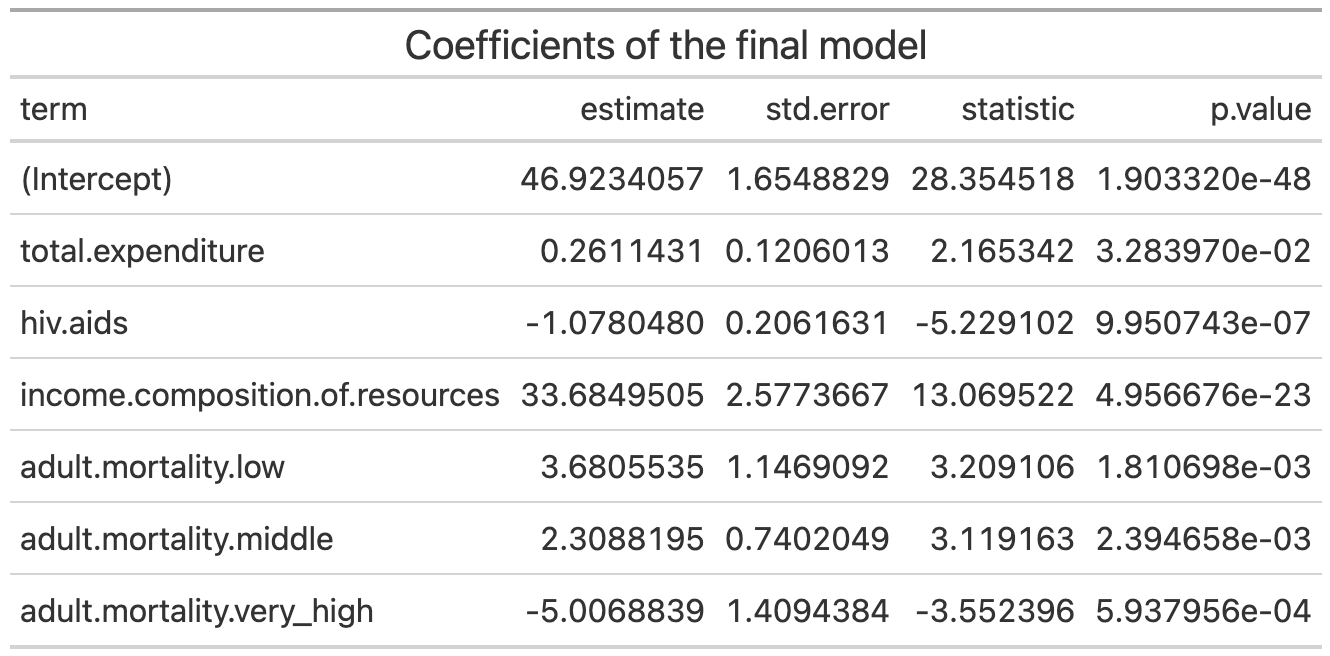
\includegraphics{figures/coefficients/coeff-model.png}
	\caption{Coefficients of the model}
	\label{fig:coeff-model}
\end{figure}

Looking at the p-values, all the coefficients $\beta_k$ are statistically significants at a significance level of $\alpha = 0.05$.

We can interpret the different coefficients the following way,
\begin{itemize}
	\item An increase of $1\%$ in the governement expenditure on health (as a percentage of total expenditure) leads to an increase of $0.26\%$ of life expectancy.
	\item An increase of $1$ death caused by HIV/AIDS for people under $5$ years old per $1000$ births leads to a decrease of $1.07/1000$ of life expectancy.
	\item An increase of ...
	\item Having a low adult mortality leads to an incrase of $3.6$ years of life expectancy.
	\item Having a middle adult mortalty leads to an increase of $2.3$ years of life expectancy.
	\item Having a very high adult mortality leads to a decrease of $5$ years of life expectancy.
\end{itemize}